\section{Development Methodology}\label{Development Methodology} 
    We did not follow any established development methodology, such as \gls{scrum}\footnote{\gls{scrum} - An agile software development methodology. [\url{http://en.wikipedia.org/wiki/Scrum_(development)}]} or \gls{xp}\footnote{\gls{xp} - A type of agile software development. [\url{http://en.wikipedia.org/wiki/Extreme_programming_practices}]}, as this project required more planning and configuration of existing solutions, than actual coding. In the process of choosing a development methodology we considered scrum, waterfall, agile, xp, and some others in addition to combination of these. In the end we chose a mix of the \gls{waterfall}\footnote{\gls{waterfall} - A sequential design process. [\url{http://en.wikipedia.org/wiki/Waterfall_development}]} and \gls{agile}\footnote{\gls{agile} - A group of software development methodologies based on iterative and incremental development. [\url{http://en.wikipedia.org/wiki/Agile_software_development}]}, we discuss these decisions in the sections below. You will also 
find a list of the tools we chose to work with, and why we decided to use them. 
    
    Because this was a research project, the customer would act more as an advisor than a customer, and would have more suggestions and advice than demands and requirements. We had been given a clear understanding of what the final product should be, and we had a list of requirements that would be met. Other than that, we were relatively free regarding how we go about solving the problem. Because of this, a single methodology, like Scrum, wouldn't work for us, as it would require us to be in close and frequent contact with the customer, presenting a prototype at regular intervals, and continue development based on the customers feedback and demands.
    
    As mentioned, this was a project that required quite a lot of planning before any programming could be done. This necessitated that we started the development according to a waterfall model in terms of the architecture planning, as well as the requirements specification. By using the waterfall model in these first phases, we ensured that the planning was done thoroughly in order to minimize the amount of trial and error during the later implementation phase.
    
    As the project progressed we switched to a more agile development method, in order to allow iterative development and facilitate necessary changes that have turned up as code was produced, as opposed to waterfall-coding, where we would have to strictly follow our plans. Agile also let us use the flat organizational structure we had chosen, which we believed would greatly help cooperation within the team.
    
    \subsection{Project Organization}\label{Project Organization}
    
    We divided the project tasks into work packages. These packages are represented in a \gls{wbs}\footnote{\gls{wbs} - An oriented decomposition of a project into smaller components. [\url{http://en.wikipedia.org/wiki/Work_breakdown_structure}]} (ref:~\ref{Work Breakdown Structure}). The schedule for the project is represented in a \gls{gantt}\footnote{\gls{gantt} - A type of bar chart that illustrates a project schedule. [\url{http://en.wikipedia.org/wiki/Gantt}]} (Fig:~\ref{fig:gantt}). The figure is part of our full Gantt chart. As the full diagram cannot be included nicely in the report we have attached it as an HTML document (ref:~\ref{File Attachments}).
     
        \begin{figure}[h]
            \centering
            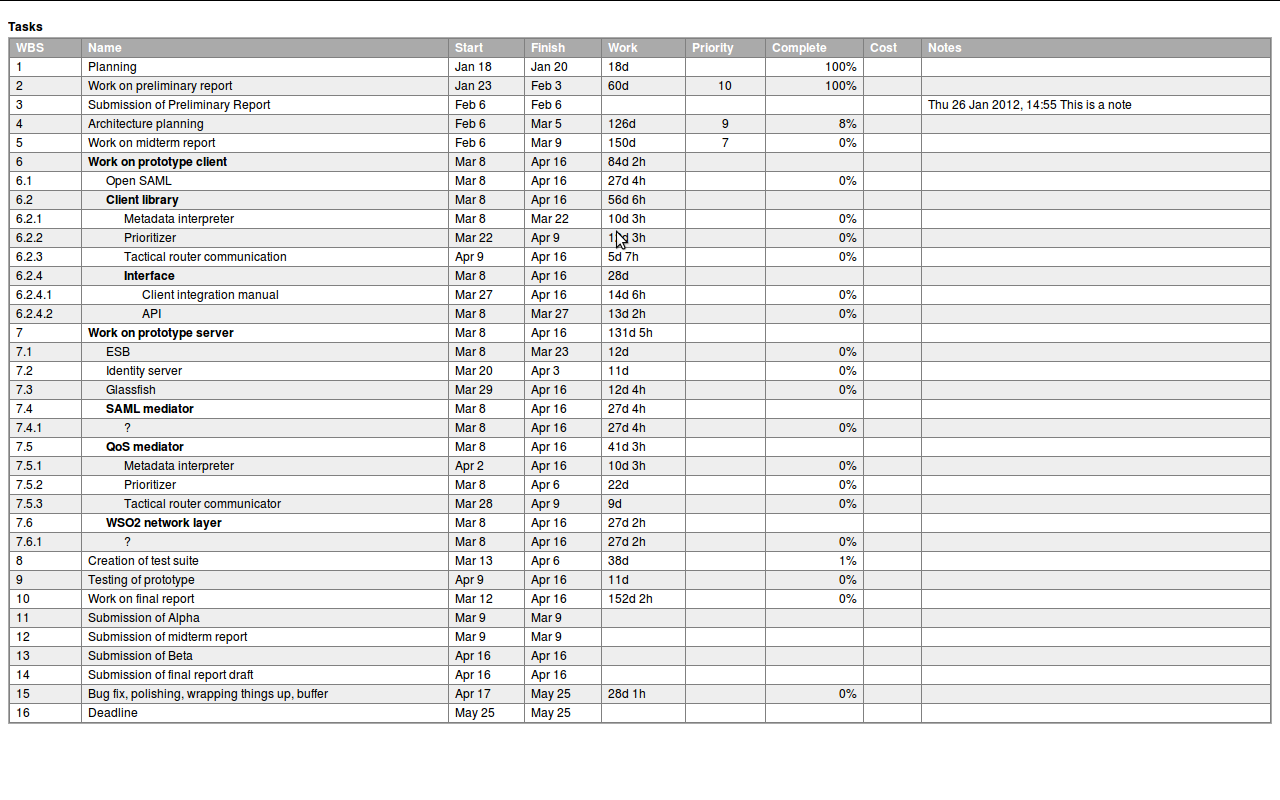
\includegraphics[width=\textwidth]{gantt}
            \caption{Part of our Gantt diagram} 
            This is an example to show that the gantt diagram exists and what it looks like. Se full diagram under file attachments (ref:~\ref{File Attachments}).
            \label{fig:gantt}
        \end{figure}
    
    \subsection{Software project life cycle}\label{Software project life cycle}
    
    For our project life cycle we chose agile. Originally we started out with the intention of using Scrum and Scrum only. That idea was quickly scrapped as we found out that our task was very research heavy. This made us rethink our approach to the development cycle and turn in the direction of agile software development.
    
    Early in the project we expected that we could begin coding and prototyping before too long. This proved to be wrong as there was a lot of research to be done. Scrum was originally a tactic to improve product flexibility and production speed. This works very well in software development when you already know what you are supposed to do and the major part of the task is to implement the required functionality. When the functionality has to be designed and researched extensively, scrum becomes unsuitable. 
    
    With the agile method there are elements that suits us better than others. "Individuals and Interaction" and "Customer Collaboration" are two important elements that we use. The full description of the agile method can be found in the Agile Manifesto\footnote
        {Agile Manifesto, the key elements of the agile software development method. [\href{http://http://agilemanifesto.org/}{AgileManifesto.org}]}.
    
    "Individuals and interactions" is strongly connected with the organization of our team (ref:~\ref{Team Organization}). The flat team structure forced us to have a good dialog among the group members. This increased the team members' interaction and strengthens the team communication. The strengthened communication promotes the individuals of the group and the team members' confidence, which in turn increases the total productivity of the group. The frequent interactions with the customer are also a part of our adaption to the agile development method. 
    
    "Customer Collaboration" is the aspect of the group contacting the customer and keeping a good dialog with them. This was to make sure that we produced the product that the customer wanted. To achieve this part of the agile manifesto we had meetings with the customer every week, and had frequent email correspondence to iron out the bumps in our product. The frequent communication with the customer helped us to create a more precise and consistent system with better documentation. The main part of the communication with the customer was for the benefit of the project, and constant improvement. The constant improvement and iterative work flow is a central part of the agile method. 
    
    Scrum is an agile development methodology. Waterfall is not. Waterfall takes development very much a step at a time. While agile-like approaches like scrum run around a track, repeating its steps over and over. The common steps of waterfall and scrum agile are: planning, build, test, review, deploy. 
               
    Scrum does these steps in an iterative manner. First planning, building, testing and then review. These steps are repeated several times before another bigger review is done, followed by testing. This cycle repeats over and over, until the project is done. 
    
    Waterfall  does these steps one at a time. First the planning part until all the planning is complete. Then the implementation part where all the coding is done. Testing follows as a natural step. The testing is thorough, so that no more coding or testing has to be done. Then the review part follows, where functionality, requirements and completeness is assessed. And deployment comes as the last step, when everything is working as it should and everything else is complete.  
    
    We ended up using something like iterative waterfall. Where we planned a lot in the beginning, started coding and testing nearly at the same time, the testing consisting of unit tests at that stage. While coding we had reviews and a bit of quality control of the code. When the code was complete we started system testing. System testing and code improvement went in iterations as we found problems and mistakes that were overlooked before. Then we followed with the documentation part, representing a sort of deployment phase of the waterfall methodology. 

    \subsection{System Technology}\label{System Technology}
    
    To begin with we intended to use \gls{junit}\footnote{\gls{junit} - A testing framework for the Java programming language. [\url{http://junit.org/}]} tests throughout the project. This started well in the implementation phase, but faded away towards the end of the implementation phase; especially when the implementation was a week delayed and we used a lot of time debugging and making the system actually work. 
    
    At the beginning we planned to have code reviews and go through all the code and fix code deficiencies. This was meant to happen every other week. As good as this intention is we didn't manage to do it as often as we would like. In the server side we had two code reviews. With the client we had none. We also experienced that the code reviews didn't really work out as we had planned. While debugging the client library and the server side of the developed application we found a lot of bugs and logic errors after the code reviews. This means that our code reviews were bad and that they didn't really fulfil their purpose. 
    
    One of our requirements was that the system should be thoroughly tested. To accomplish this requirement we decided to use the MobiEmu framework. MobiEmu is a network emulator that emulates network traffic and behaviour. It is based on NS3 and can test multiple nodes in a virtual network. This gives us the advantage of testing our system to a good extent of the real time battle situation that the system is thought to operate in. Another reason that we used this testing framework is that one of our group members had previous experience with it. The testing framwork gave us useful test results that are discussed in section~\ref{Testing}.

    Furthermore we used \gls{git}\footnote{\gls{git} - A free and open source, distributed version control system. [\url{http://www.git-scm.com}]} and \gls{github}\footnote{\gls{github} - A web-based hosting service for software development projects that use the Git version control system. [\url{http://www.github.com}]} to handle our files and repository. 
    
    Along with git we used Google-docs, now drive, to store and share documents. This helped us greatly in the cooperation of this project. Google docs allowed us to be multiple people to working on the same document at the same time. 
    
    \gls{latex}\footnote{\gls{latex} - A document preparation system for the \TeX -typesetting program} is obviously the preferred report scripting language for the task of writing this report. Latex helped us a lot in the report writing process. Syntax highlighting, easy integration of figures and good structure to the report files are examples of benefits we got from using \Tex.
    
    With input from the customer and their approval we decided to use Apache2 license for our code. As far as all parties could find, there was no negative side for any of us. 

    As for the personal development environment, the individual person was responsible to get his system to work. While the choice of environment is free we presume that we achieved greater productivity than if everyone were forced to use the same environment, e.g: ubuntu with eclipse.  

    As for a total list of tools that was use, see the section about Tested tools, (ref:~\ref{toolslist})    
    
